\section{Model Card per Support Vector Machine (SVM)}

\subsection{Informació General}
\begin{itemize}

\item \textbf{Nom del model}: SVM per a la predicció de l'estatus de pacients amb Cirrosi Hepàtica.
\item \textbf{Tipus de model}: Support Vector Machine (SVM).
\item \textbf{Font}: model general extret de la llibreria scikit-learn de Python.
\item \textbf{Desenvolupadors}: Cai Selvas Sala, estudiant del Grau en Intel·ligència Artificial de la Universitat Politècnica de Catalunya.
\item \textbf{Data de creació}: 28/12/2023
\item \textbf{Versió del model}: 1.0
\item \textbf{Descripció del Model}: El SVM és un model de classificació utilitzat per a predir l'estatus (`Alive', `Dead', `LiverTransplant') de pacients amb Cirrosi Hepàtica. Utilitza un kernel lineal per a separar les classes i ha estat entrenat amb un conjunt de dades que inclouen variables clíniques i demogràfiques.
\end{itemize}

\subsection{Hiperparàmetres}
Han estat determinats mitjançant una validació creuada amb \textit{K-Fold} ($k = 5$).
\begin{itemize}
	\item \textbf{Kernel}: s'ha utilitzat un kernel lineal.
	\item \textbf{C}: s'ha utilitzat el valor $C = 5$. No es recomana, però es pot modificar si es desitja.
	\begin{figure}[H]
	\centering
	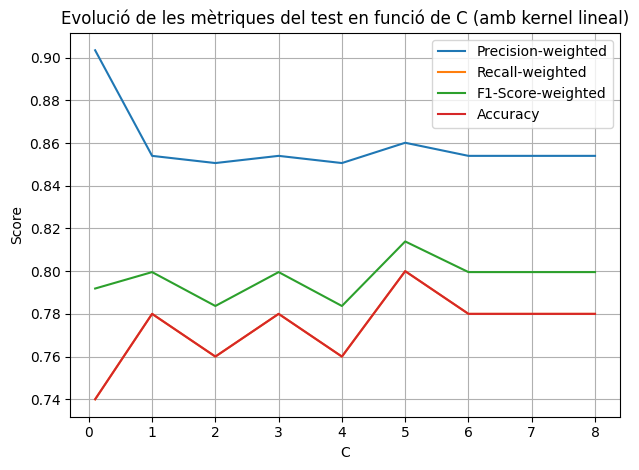
\includegraphics[width=0.5\linewidth]{img/c_evolution.png}
	\caption*{Evolucició de les mètriques en el test en funció del paràmetre C. \textit{Precision-weighted} i \textit{recall-weighted} es solapen en la gràfica, van junts.}
	\end{figure}
\end{itemize}

\subsection{Dades}
\begin{itemize}
\item \textbf{Font de les dades}: Estudi de Mayo Clinic sobre Cirrosis \cite{misc_cirrhosis_patient_survival_prediction_878}.
\item \textbf{Període de recopilació}: 1974 - 1948.
\item \textbf{Número de mostres inicials}: 418 pacients.
\item \textbf{Preprocessament}:
\begin{itemize}
	\item \textbf{Particionat en train i test}: 85\% train i 15\% test (amb el mètode \textit{stratify} per mantenir la distribució de classes).
	\item \textbf{Tractament d'outliers}: no s'han eliminat outliers.
	\item \textbf{Tractament de missings}: 
	\begin{itemize}
		\item \textbf{Eliminació de mostres}: no s'han considerat les mostres amb 9 valors faltants per garantir una millor qualitat de les dades.
		\item \textbf{Imputació de missings}: KNN Imputer ($k=15$) per variables numèriques. Random Forest Classifier (amb criteri `gini') per categoòriques.
	\end{itemize}
	\item \textbf{Codificació de variables}: variables categòriques codificades mitjançant \textit{Ordinal Encoding}.
	\item \textbf{Escalat de variables}: variables numèriques escalades a través de \textit{MinMax Scaler}.
	\item \textbf{Balanceig de classes}: mètode \textit{SMOTE} per a balancejar les classes de la variable objectiu (\textit{Status}). Amb això, el dataset d'entrenament consta de 441 mostres (pacients).
	\item \textbf{Característiques incloses}: Edat, Sexe, Resultats de laboratori (Presència o quantitat de Ascites, Hepatomegaly, Spiders, Edema, Cholesterol, Albumin, Copper, Alk\_Phos, SGOT, Tryglicerides, Platelets, Prothrombin), estat de la malaltia (Stage), dies del pacient en el tractament, administració del tractament o placebo, estat final del pacient.

\end{itemize}
\end{itemize}

\subsection{Validació}
\begin{itemize}
\item \textbf{Mida del conjunt de test}: 50 mostres (pacients). 
\item \textbf{Rendiment}:
\begin{itemize}
	\item \textbf{Rendiment mitjà en validació creuada}: F1-Score Weighted = 0,7463.
	\item \textbf{Rendiment en la validació (test)}:
	\begin{itemize}
		\item F1-Score Weighted = 0,8139.
		\item Accuracy = 0,8.
		\item Precision Weighted = 0.8601.
		\item Recall Weighted = 0.8.
	\end{itemize}
	\item Matriu de confusió:
	\begin{figure}[H]
	\centering
	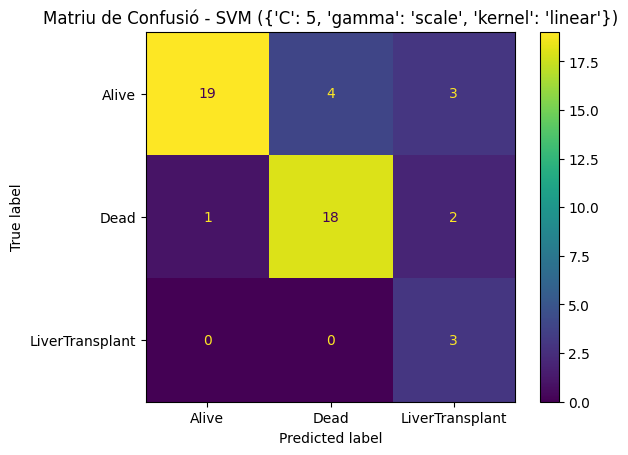
\includegraphics[width=0.6\linewidth]{img/svm-cm.png}
	\end{figure}
\end{itemize}
\end{itemize}

El rendiment pot variar segons la naturalesa del conjunt de dades de validació/test. Les prediccions de la classe `LiverTransplant' només han pogut ser provades amb les 3 mostres del conjunt de test, de manera que és difícil que es mantinguin els resultats que es mostren en la matriu de confusió. Generalment, el model tendeix a predir falsos positius en `LiverTransplant' i `Dead'.

\subsection{Advertències i Recomanacions}
Degut a desbalangeigs en atributs com ara \textit{Sex}, pot haver biaixos de sexe.

El model està dissenyat per a ser utilitzat com a eina de suport a la decisió clínica. En cap cas s'hauria d'utilitzar com a única font per a prendre decisions clíniques sensibles. Pot servir per fer una estimació de l'estat final d'un pacient amb Cirrosi per tal de prendre mesures sobre com guiar el seu tractament, però sempre sota la responsabilitat i aprovació d'un metge o professional especialitzat.

\subsection{Limitacions}
\begin{itemize}
\item Per funcionar correcatment amb dades externes, aquestes s'han de preprocessar de la mateixa manera en què el model ha estat entrenat.
\item EL model no és totalment precís, en certs casos pot predir una classe que no és correcta, tal i com es veu en la matriu de confusió.
\item El model pot tenir lleuger overfitting, de maner que els resultats siguin pitjors en un escenari real.
\end{itemize}

%-------------------------------------------------------------------------------------